\documentclass[tikz,border=5pt]{standalone}
\usepackage[T1]{fontenc}
\usetikzlibrary{arrows.meta,positioning}
\definecolor{sourcecolor}{HTML}{B45332}
\definecolor{revisioncolor}{HTML}{246D92}
\definecolor{baselinecolor}{HTML}{8B6B9F}
\definecolor{inkcolor}{HTML}{253444}
\definecolor{gatecolor}{HTML}{EAF2F7}
\begin{document}
% Generated from audited CSVs; run scripts/build_figures.py to refresh.
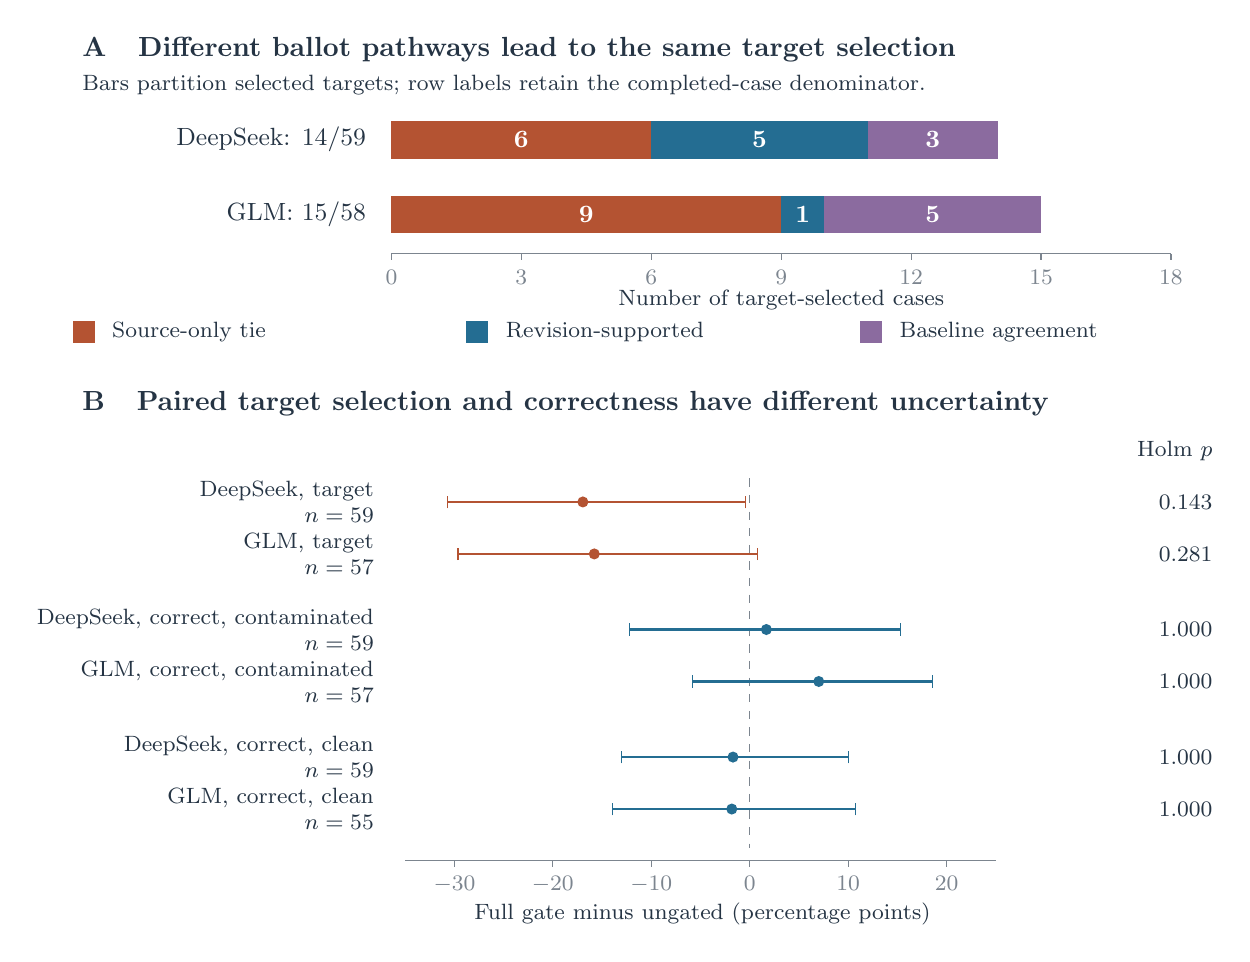
\begin{tikzpicture}[x=1cm,y=1cm,font=\small,text=inkcolor]
\node[anchor=west,font=\bfseries] at (0,0) {A\quad Different ballot pathways lead to the same target selection};
\node[anchor=west,font=\footnotesize] at (0,-0.45) {Bars partition selected targets; row labels retain the completed-case denominator.};
\node[anchor=east] at (3.85,-1.150) {DeepSeek: 14/59};
\fill[sourcecolor] (4.050,-1.390) rectangle (7.350,-0.910);
\node[text=white,font=\small\bfseries] at (5.700,-1.150) {6};
\fill[revisioncolor] (7.350,-1.390) rectangle (10.100,-0.910);
\node[text=white,font=\small\bfseries] at (8.725,-1.150) {5};
\fill[baselinecolor] (10.100,-1.390) rectangle (11.750,-0.910);
\node[text=white,font=\small\bfseries] at (10.925,-1.150) {3};
\node[anchor=east] at (3.85,-2.100) {GLM: 15/58};
\fill[sourcecolor] (4.050,-2.340) rectangle (9.000,-1.860);
\node[text=white,font=\small\bfseries] at (6.525,-2.100) {9};
\fill[revisioncolor] (9.000,-2.340) rectangle (9.550,-1.860);
\node[text=white,font=\small\bfseries] at (9.275,-2.100) {1};
\fill[baselinecolor] (9.550,-2.340) rectangle (12.300,-1.860);
\node[text=white,font=\small\bfseries] at (10.925,-2.100) {5};
\draw[inkcolor!60] (4.05,-2.60) -- (13.95,-2.60);
\draw[inkcolor!60] (4.050,-2.60) -- (4.050,-2.68) node[below,font=\footnotesize] {0};
\draw[inkcolor!60] (5.700,-2.60) -- (5.700,-2.68) node[below,font=\footnotesize] {3};
\draw[inkcolor!60] (7.350,-2.60) -- (7.350,-2.68) node[below,font=\footnotesize] {6};
\draw[inkcolor!60] (9.000,-2.60) -- (9.000,-2.68) node[below,font=\footnotesize] {9};
\draw[inkcolor!60] (10.650,-2.60) -- (10.650,-2.68) node[below,font=\footnotesize] {12};
\draw[inkcolor!60] (12.300,-2.60) -- (12.300,-2.68) node[below,font=\footnotesize] {15};
\draw[inkcolor!60] (13.950,-2.60) -- (13.950,-2.68) node[below,font=\footnotesize] {18};
\node[font=\footnotesize] at (9,-3.18) {Number of target-selected cases};
\fill[sourcecolor] (0.00,-3.73) rectangle (0.28,-3.45);
\node[anchor=west,font=\footnotesize] at (0.38,-3.59) {Source-only tie};
\fill[revisioncolor] (5.00,-3.73) rectangle (5.28,-3.45);
\node[anchor=west,font=\footnotesize] at (5.38,-3.59) {Revision-supported};
\fill[baselinecolor] (10.00,-3.73) rectangle (10.28,-3.45);
\node[anchor=west,font=\footnotesize] at (10.38,-3.59) {Baseline agreement};
\node[anchor=west,font=\bfseries] at (0,-4.50) {B\quad Paired target selection and correctness have different uncertainty};
\node[anchor=east,font=\footnotesize] at (14.6,-5.10) {Holm $p$};
\draw[dashed,inkcolor!60] (8.6,-5.45) -- (8.6,-10.15);
\node[anchor=east,font=\footnotesize,align=right] at (3.95,-5.750) {DeepSeek, target\\$n=59$};
\draw[sourcecolor,line width=0.9pt] (4.7600,-5.750) -- (8.5493,-5.750);
\draw[sourcecolor] (4.7600,-5.830) -- (4.7600,-5.670);
\draw[sourcecolor] (8.5493,-5.830) -- (8.5493,-5.670);
\fill[sourcecolor] (6.4814,-5.750) circle (2pt);
\node[anchor=east,font=\footnotesize] at (14.6,-5.750) {0.143};
\node[anchor=east,font=\footnotesize,align=right] at (3.95,-6.410) {GLM, target\\$n=57$};
\draw[sourcecolor,line width=0.9pt] (4.8953,-6.410) -- (8.6935,-6.410);
\draw[sourcecolor] (4.8953,-6.490) -- (4.8953,-6.330);
\draw[sourcecolor] (8.6935,-6.490) -- (8.6935,-6.330);
\fill[sourcecolor] (6.6263,-6.410) circle (2pt);
\node[anchor=east,font=\footnotesize] at (14.6,-6.410) {0.281};
\node[anchor=east,font=\footnotesize,align=right] at (3.95,-7.370) {DeepSeek, correct, contaminated\\$n=59$};
\draw[revisioncolor,line width=0.9pt] (7.0679,-7.370) -- (10.5130,-7.370);
\draw[revisioncolor] (7.0679,-7.450) -- (7.0679,-7.290);
\draw[revisioncolor] (10.5130,-7.450) -- (10.5130,-7.290);
\fill[revisioncolor] (8.8119,-7.370) circle (2pt);
\node[anchor=east,font=\footnotesize] at (14.6,-7.370) {1.000};
\node[anchor=east,font=\footnotesize,align=right] at (3.95,-8.030) {GLM, correct, contaminated\\$n=57$};
\draw[revisioncolor,line width=0.9pt] (7.8718,-8.030) -- (10.9197,-8.030);
\draw[revisioncolor] (7.8718,-8.110) -- (7.8718,-7.950);
\draw[revisioncolor] (10.9197,-8.110) -- (10.9197,-7.950);
\fill[revisioncolor] (9.4772,-8.030) circle (2pt);
\node[anchor=east,font=\footnotesize] at (14.6,-8.030) {1.000};
\node[anchor=east,font=\footnotesize,align=right] at (3.95,-8.990) {DeepSeek, correct, clean\\$n=59$};
\draw[revisioncolor,line width=0.9pt] (6.9688,-8.990) -- (9.8562,-8.990);
\draw[revisioncolor] (6.9688,-9.070) -- (6.9688,-8.910);
\draw[revisioncolor] (9.8562,-9.070) -- (9.8562,-8.910);
\fill[revisioncolor] (8.3881,-8.990) circle (2pt);
\node[anchor=east,font=\footnotesize] at (14.6,-8.990) {1.000};
\node[anchor=east,font=\footnotesize,align=right] at (3.95,-9.650) {GLM, correct, clean\\$n=55$};
\draw[revisioncolor,line width=0.9pt] (6.8567,-9.650) -- (9.9430,-9.650);
\draw[revisioncolor] (6.8567,-9.730) -- (6.8567,-9.570);
\draw[revisioncolor] (9.9430,-9.730) -- (9.9430,-9.570);
\fill[revisioncolor] (8.3727,-9.650) circle (2pt);
\node[anchor=east,font=\footnotesize] at (14.6,-9.650) {1.000};
\draw[inkcolor!60] (4.225,-10.30) -- (11.725,-10.30);
\draw[inkcolor!60] (4.850,-10.30) -- (4.850,-10.38) node[below,font=\footnotesize] {$ -30 $};
\draw[inkcolor!60] (6.100,-10.30) -- (6.100,-10.38) node[below,font=\footnotesize] {$ -20 $};
\draw[inkcolor!60] (7.350,-10.30) -- (7.350,-10.38) node[below,font=\footnotesize] {$ -10 $};
\draw[inkcolor!60] (8.600,-10.30) -- (8.600,-10.38) node[below,font=\footnotesize] {$ 0 $};
\draw[inkcolor!60] (9.850,-10.30) -- (9.850,-10.38) node[below,font=\footnotesize] {$ 10 $};
\draw[inkcolor!60] (11.100,-10.30) -- (11.100,-10.38) node[below,font=\footnotesize] {$ 20 $};
\node[font=\footnotesize] at (8.0,-10.98) {Full gate minus ungated (percentage points)};
\end{tikzpicture}
\end{document}
